
%%正文页
\newpage
\setcounter{page}{1}

\section{介绍}

自1950年来,确定性有限自动机的最小化就一直在研究当中。简单来说就是找到一个唯一的(直至同构)最小的确定性有限自动机,它能接收与给定的确定性有限自动机相同的语言。解决这一问题的算法应用范围很广,从编译器构造到硬件电路的最小化都有它的身影。有了形式多样的应用程序,不同的表示形式的数量也在增加:大多数教科书都有自己的变体,而时间复杂度最优的算法 (Hopcroft的算法) 仍然晦涩难懂。

本文介绍了有限自动机最小化算法的有关分类。如下所示:

\begin{itemize}
    \item[·] 大多数教材的作者称他们的最小化算法由 Huffman 算法 \cite{Huff54} 和 Moore 算法 \cite{Moor56} 直接推导得到。不幸的是,大多数教材都展示了截然不同的算法 (比如 \cite{AU92,ASU86,Hu79,Wood87}), 只有由 Aho 和 Ullman 发表的算法直接源自 \cite{Huff54, Moor56}。
    \item[·] 虽然大多数算法依赖于计算状态的等价关系,但伴随算法演示的许多解释并未明确提及算法是计算等价关系、它包含的状态划分还是它的补充。
    \item[·] \uline {Comparison of the algorithms is further hindered by the vastly differing styles of presentation --- sometimes as imperative programs or as functional programs, but frequently only as a descriptive paragraph. 算法之间的比较进一步受到呈现方式的巨大差异的阻碍。有时作为命令式程序或函数式程序,但通常只作为描述性段落。}
\end{itemize}
A related taxonomy of finite automata construction algorithms appears in [Wats93].\\
有限自动机构造算法的相关分类在\cite{Wats93}中。

\uline{All except one of the algorithms rely on determining the set of automaton states which are equivalent.} The algorithm that does not make use of equivalent states is discussed in Section 2. In Section 3 the definition and some properties of equivalence of states is given. Algorithms that compute equivalent states are presented in Section 4. The main results of the taxonomy are summarized in the conclusions Section 5. Appendices A and B give the basic definitions required for reading this paper. The definitions related to finite automata are taken from [Wats93]. The minimization algorithm relationships are shown in a "family" tree\ in Figure 1.

\uline{除了一个算法之外,其他所有算法依赖于确定等价}\footnote{状态的等价稍后定义。}\uline{的自动机状态的集合。}在第2节中讨论了不使用等价状态的算法。在第3节中给出了状态等价的定义和一些性质。计算等效状态的算法在第4节中给出。分类的主要结果被总结在结论部分5中。附录A和附录B给出了阅读本文所需的基本定义。与有限自动机相关的定义取自\cite{Wats93}。图1中的“Family tree”展示了最小化算法之间的关系。

The principal computation in most minimization algorithms is the determination of equivalent (or inequivalent) states —— thus yielding an equivalence relation on states. In this paper,we consider the following minimization algorithms:

大多数最小化算法的主要计算是确定等价的(或不等价的)状态,从而在状态上产生等价关系。在本文中,我们考虑以下最小化算法:

\begin{itemize}
    \item[·] Brzozowski's (possibly nondeterministic) finite automaton minimization algorithm as presented in [Brzo62]. This elegant algorithm (Section 2) was originally invented by Brzozowski, and has since been re-invented without credit to Brzozowski. Given a (possibly nondeterministic ) finite automaton without E-transitions, this algorithm produces the minimal deterministic finite automaton accepting the same language.
    
    Brzozowski(可能是非确定性的)有限自动机最小化算法 在 \cite{Brzo62} 中提出。这个优雅的算法(第2节)最初是由Brzozowski提出,此后又在没有Brzozowski的“参与”的情况下被重新提出。在没有 $\epsilon$-转移 的情况下,给出了一个(可能不确定的)有限自动机,该算法生成一个最小的接受相同的语言的确定性有限自动机。

    \item[·] Layerwise computation of equivalence as presented in [Wood87, \cite{Moor56} Brau88, Urba89]. This algorithm (Algorithm 4. 2) is a straightforward implementation suggested by the approximation sequence arising from the fixed-point definition of equivalence of states. 

    分层等价计算等价于 \cite{Wood87, Moor56, Brau88, Urba89} 中提出。算法(算法 4.2)是由状态等价的定点定义产生的近似序列所建议的直接实现。

    \item[·] Unordered computation of equivalence This algorithm (Algorithm 4.3, not appearing in the literature) computes the equivalence relation; pairs of states (for consideration of equivalence) are chosen in an arbitrary order.

    等价无序计算。该算法(算法4.3,未出现在文献中)计算等价关系;以任意顺序选择状态对(考虑等价性)。

    \item[·] Unordered computation of equivalence classes as presented in [ASU86]. This algorithm (Algorithm 4.4)is a modification of the above algorithm computing equivalence of states.

    等价类的无序计算发表在\cite{ASU86}。该算法(算法4.4)是上述算法计算状态等价性的一种更改。

\end{itemize}

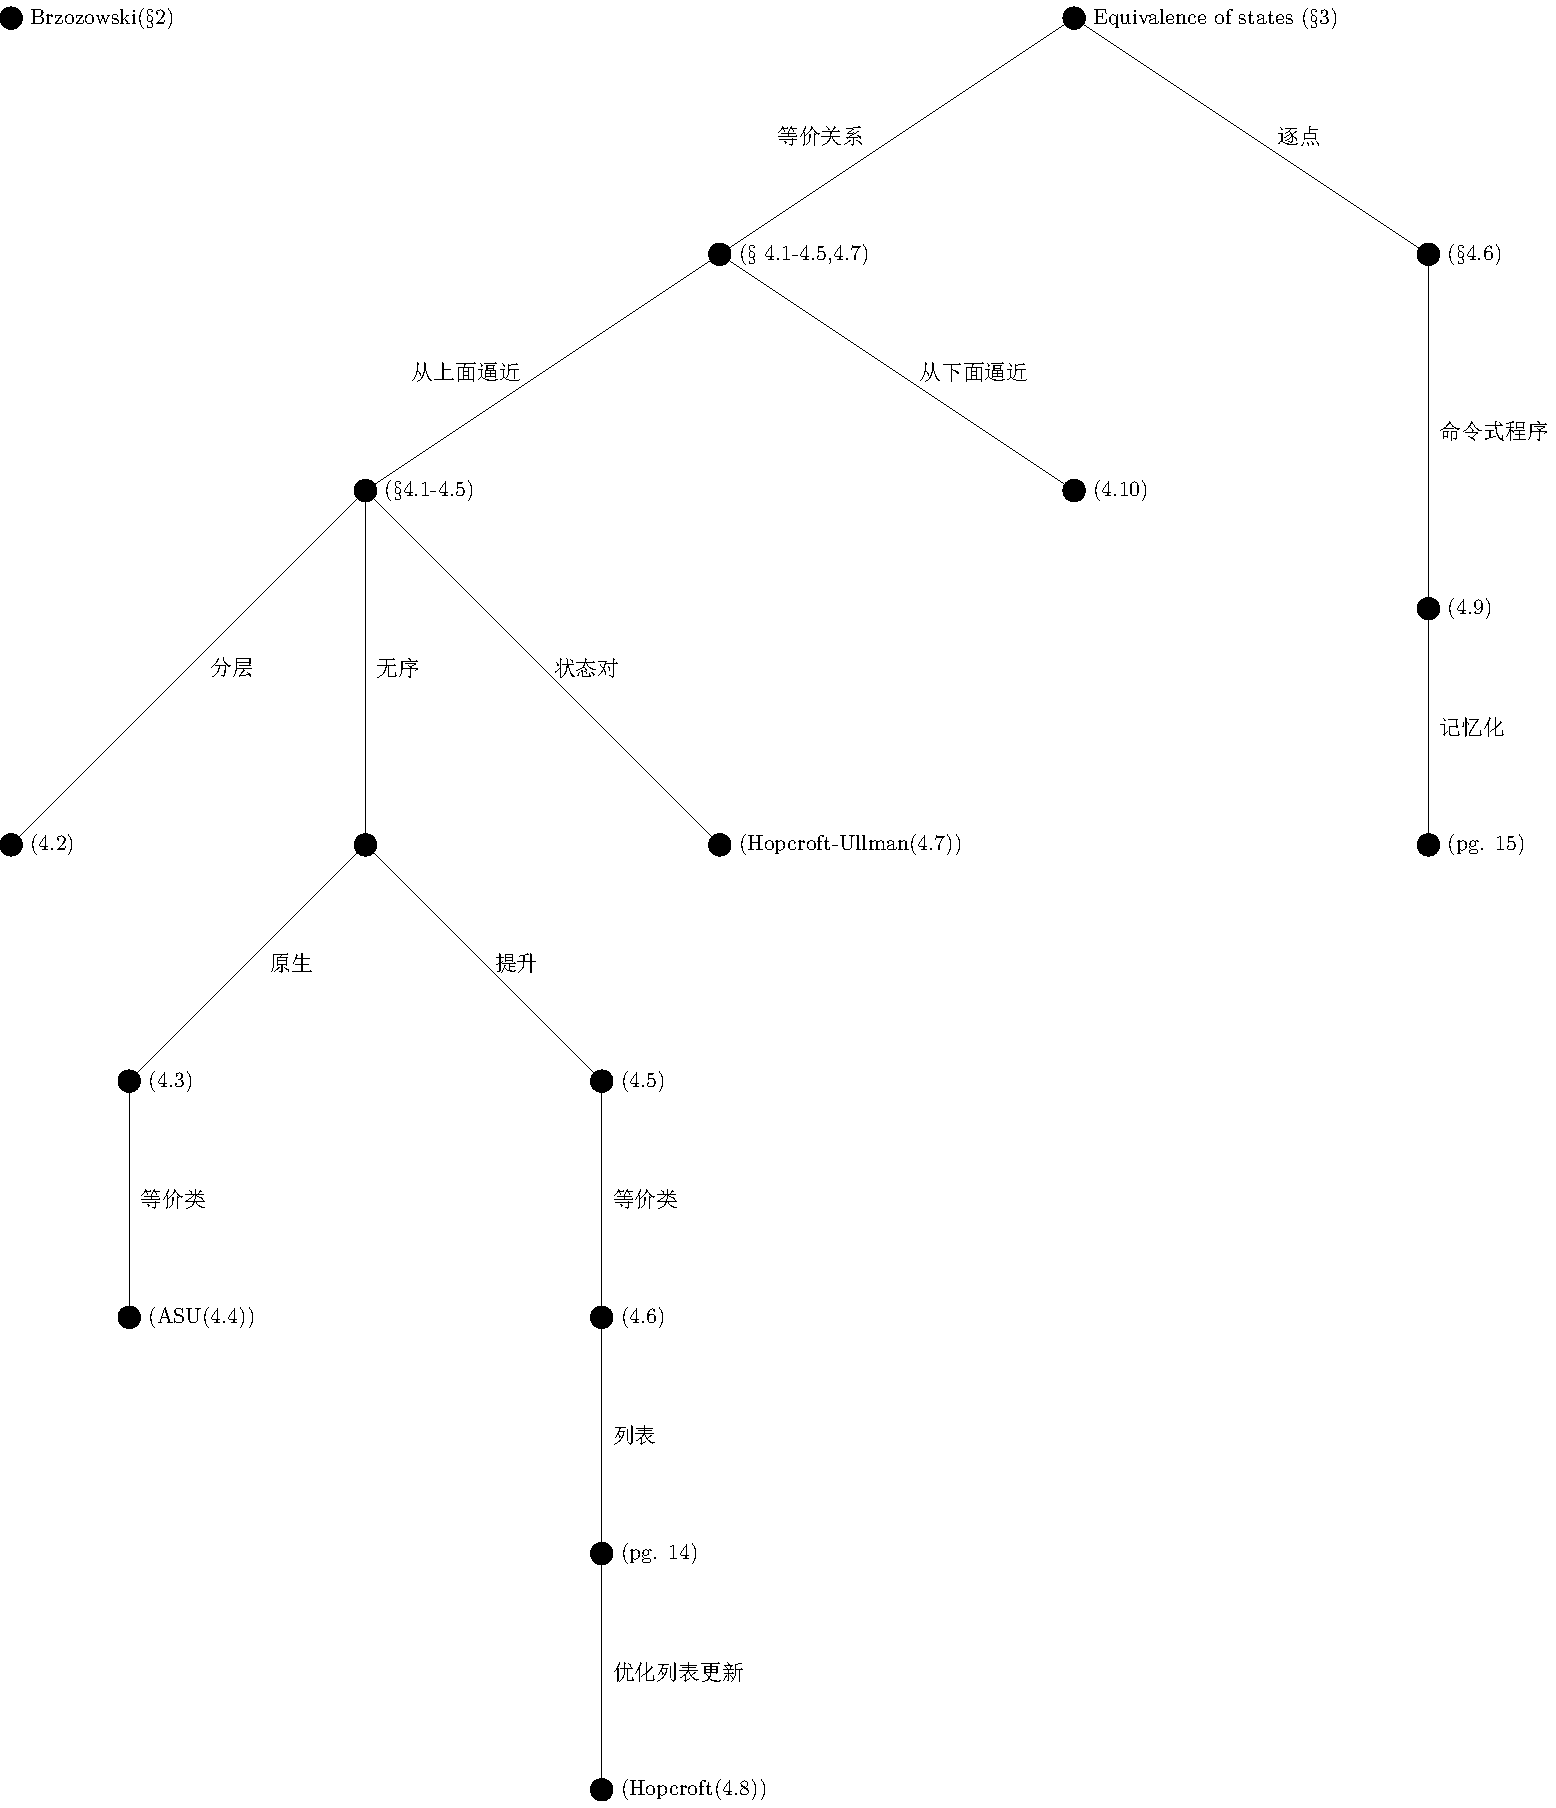
\includegraphics[width =.93\textwidth]{figure1.pdf}

Figure 1: The family trees of finite automata minimization algorithms. Brzozowski's minimization algorithm is unrelated to the others, and appears as a separate(single vertex)tree. Each algorithm presented in this paper appears as a vertex in this tree. For each algorithm that appears explicitly in this paper, the construction number appears in parentheses(indicating where it appears in this paper). For algorithms that do not appear explicitly, a reference to the section or page number is given. Edges denote a refinement of the solution (and therefore explicit relationships between algorithms). They are labeled with the name of the refinement.

图1:有限自动机最小化算法的“Family tree”。Brzozowski的最小化算法与其他算法无关,并作为一个单独的(单顶点)树出现。本文提出的每一个算法都作为树的顶点出现。对于本文中明确出现的每个算法,构造数在括号中(标示它在本文中出现的位置)。对于未显式显示的算法,给出了相应的页码。边表示解的\uline{细化}(也即算法之间的显式关系)。它们被标记为\uline{细化}的名称。

\begin{itemize}

    \item[·] Improved unordered computation of equivalence. This algorithm (Algorithm 4.5, not appearing in the literature) also computes the equivalence relation in all arbitrary order. The algorithm is a minor improvement over the other unordered algorithm.
 
    改进的等价的无序计算。这个算法(算法4.5,没有出现在文献中)也以任意顺序计算等价关系。该算法是对其他无序算法的一个小改进。

    \item[·] Improved unordered computation of classes. This algorithm (Algorithin 4.6, not appearing in the literature) is a modification of the above algorithm to compute the equivalence classes of states. This algoritm is used in the derivation of Hopcroft's minimization algorithin.
 
     改进了类的无序计算。该算法(算法4.6,不在文献中)是上述算法的修改,用来计算等价类的状态。该算法用于Hopcroft最小化算法的推导。

    \item[·] Hopcroft and Ullman's algorithm as presented in [HU79]. This algorithm (Algorithm 4.7) computes the inequivalence (distinguishability) relation. Although it is based upon the algorithus of Huffinan and Moore [Huff54, Moor 56], this algorithm uses some interesting encoding techniques.
 
    Hopcroft 和 Ullman 算法在\cite{Hu79}中提出。该算法(算法4.7)计算不等价(区分性)关系。虽然它是基于 Huffinan \cite{Huff54}和 Moore \cite{Moor56} 的算法,但该算法使用一些有趣的编码技术。

    \item[·] Hopcroft's algorithm as presented in [Hopc71, Grie73]. This algorithm (Algorithm 4.8)is the best known algorithm (in terms of running time analysis) for minimization. As the original presentation by Hopcroft is diflicult to understand, the presentation in this paper is based upon the one giveu by Gries.
 
    HopRofft的算法在 \cite{Hopc71, Grie73} 提出 。该算法(算法4.8)是用于最小化的最有名的算法(在运行时间分析方面)。由于 Hopcroft 的原始陈述是难以理解的,本文的介绍基于Gries的文章。

    \item[·] Pointwise computation of equivalence. This algorithm (Algorithm 4.9 not appearing in the literature) computes the equivalence of a given pair of states. It draws upon some nonautomata related techniques, such as: structural equivalence of types and memoization of functional programs.
 
    等价的点态计算。该算法(算法4.9,不在文献中)计算给定状态对的等价性。它借鉴了一些非自动机相关的技术,例如:类型的结构等价和函数式程序的记忆化。

    \item[·] \uline{Computation of equivalence from below (with respect to refinement). This algorithm (Algorithm 4.10, not appearing in the literature) computes the equivalence relation from below. } Unlike any of the other known algorithms, the intermediate result of this algorithm can be used to construct a smaller (although not minimal) deterministic finite automaton.
  \newline
    \uline{由下面的内容(关于细化)计算等价性。该算法(算法4.10,不在文献中)计算从下面的等价关系。}与任何其他已知算法不同,该算法的中间结果可用于构造较小的(虽然不是最小的)确定性有限自动机。

\end{itemize}